\section{설계}
\label{sec:ldu}

%$$$$$$$$$$$$$$$$$$$$$$$$$$$$$$$$$$$$$$$$$$$$$$$$$$$$$$$$$$$$$$$$$$$$$$$$$$$$$$$$
%Paragraph 1: LDU의 특징을 간단한 설명과 이번장에 대한 설명(LDU의 특징을 요약하여 설명)
%$$$$$$$$$$$$$$$$$$$$$$$$$$$$$$$$$$$$$$$$$$$$$$$$$$$$$$$$$$$$$$$$$$$$$$$$$$$$$$$$
LDU는 리눅스 커널의 높은 업데이트 비율을 가진 자료구조의 확장성 문제를 해결하기 위한 동기화 방법이다.
LDU는 최소한의 하드웨어 동기화 기법을 사용한 로그 기반 방법 중 하나 이다.
기존 연구된 타임스탬프 카운터 기반의 퍼코어 로그를 활용한 동시적 업데이트 방법은 
캐시 일관성 문제를 완벽히 제거할 수 있는 장점을 가지지만, 
대부분 \textit{Clock Source}가 다른 NUMA 머신으로 구성되어 있는 매니코어 시스템에서는 
아직 타임 \textit{Clock Skew} 등이 발생할 가능성이 높기 때문에 연산의 순서가 변경될 문제가 있다.
또한 현실적으로 하드웨어적으로 동기화 타임스탬프는 NUMA 기반의 매니코어 시스템에 존재하지 않는 것이 문제이다.

이러한 문제를 해결하기 위해, LDU는 동기화된 타임스탬프 카운터를 이용하지 않고 로그 기반 방식의 
방법과 최소한의 원자적 동기화 기능을 이용 하여 설계하였다.
따라서, LDU는 동기화된 타임스탬프 카운터를 사용하는 방식의 타임스탬프 카운터를 
제거함과 동시에 캐시 일관성 트래픽을 최소화하였다.
이번 장에서는 이러한 LDU의 설계 부분에 대해서 설명한다. 

\subsection{접근법}
%$$$$$$$$$$$$$$$$$$$$$$$$$$$$$$$$$$$$$$$$$$$$$$$$$$$$$$$$$$$$$$$$$$$$$$$$$$$$$$$$
%Paragraph 4: 리눅스의 update operation의 특징을 이용한 Update-side Abosrbing 
%$$$$$$$$$$$$$$$$$$$$$$$$$$$$$$$$$$$$$$$$$$$$$$$$$$$$$$$$$$$$$$$$$$$$$$$$$$$$$$$$
먼저 LDU는 두 가지 특징 이용하여 설계를 하였다. 
첫 번째 특징은 검색 자료구조 중에서 두 가지 연산이 서로 가환성(Commutativity)이 없는 연산이라도 
연산의 결과 순서가 크게 중요하지 않는 자료구조가 존재한다는 것이다. 
예를 들어, 가령 각자 서로 다른 키를 가지고 있는 두 가지 오브젝트를 삽입하는 두 개의 
연산이 있다고 가정한다면, 이 두 가지 오브젝트를 검색 자료구조에 넣을 때 이 두 가지 연산 중 
어느 것이 먼저 삽입 되는 것은 문제가 없는 자료구조가 존재한다.  
즉, 두 개의 오브젝트는 문제 없이 삽입이 되며, 그 결과는 같다~\cite{PaulCreatingAPILWN}. 
하지만 두 연산이 같은 오브젝트를 대상으로 수행하는 연산이라면, 이것은 반드시 
순서를 지켜야 한다는 것이다.  

이러한 상황을 예를 들어 설명하기 위해, 삽입 연산은 원형과 플러스 모양인 $\oplus$로 표시하고, 
삭제 연산은 원형과 마이너스 모양인 $\ominus$으로 표시하였다.
또한 특정 메모리에서 할당된 오브젝트들은 원안에 이름으로 구별하였다.
서로 다른 색과 다른 높낮이는 서로 다른 CPU를 의미한다. 
예를 들어 CORE\#2에서 삽입 연산을 수행하는 오브젝트 B는 \inv{2}{B}과 같다.

\begin{center}
$\oplus$\inv{1}{A}, $\oplus$\inv{2}{B}, $\oplus$\inv{3}{C},$\ominus$\inv{2}{A},
$\ominus$\inv{3}{C}, $\oplus$\inv{3}{A}, $\oplus$\inv{3}{C},$\ominus$\inv{1}{C}
\end{center}

위의 연산은 5개의 삽입 연산들과 3개의 삭제 연산 그리고 3개의 CPU 그리고 3개의 오브젝트를 의미한다.
여기서 같은 오브젝트에 대해서 수행하는 $\oplus$\inv{1}{A}와 $\ominus$\inv{2}{A}는 
연산 순서가 중요한 로그이며 반드시 순서대로 실행되어야 한다.  
LDU는 이러한 연산 순서가 중요한 연산들을 업데이트 순간에 삭제하는 방법을 이용한다.
그렇게 함으로써 동기화된 타임 스탬프 카운터의 필요성을 제거하였다. 
한 가지 더 중요한 사실은 이처럼 순서가 중요한 로그들은 삭제되어도 상관 없는 로그이다. 
즉 실행 결과는 같다.
예를 들어, 삽입-삭제 연산 또는 삭제-삽입 연산의 경우,
$\oplus$\inv{1}{A}$\ominus$\inv{2}{A}, $\oplus$\inv{3}{C}$\ominus$\inv{3}{C} 
그리고 $\oplus$\inv{3}{C}$\ominus$\inv{1}{C}들은 리더가 수행하기 전에 취소되어도 상관없는 연산들이다. 
따라서 남은 로그인
\begin{center}
 $\oplus$\inv{2}{B}, $\oplus$\inv{3}{A}
\end{center}
로그들은 연산 순서가 중요하지 않는 로그이다.
이처럼 LDU는 업데이트 연산이 발생하면 연산 순서가 중요한 연산들은 업데이트 순간 제거하는 방법을 
사용하여 로그를 삭제하였다.

커널에서 사용하는 자료구조의 두 번째 특징은 업데이트 연산은 특정한 순서를 가지고 있다.
리눅스 커널의 업데이트 연산은 응용프로그램에서 사용되는 자료구조의 연산과는 다르게 
같은 오브젝트(메모리에서 할당 받은 오브젝트)에 대해서 삽입 연산이 발생하면, 
같은 오브젝트를 사용하는 다음 연산은 반드시 삭제 연산이 발생하는 특징을 가지고 있다.
그 이유는 커널의 자료구조 연산은 연산 내부에서 검색(Search), 할당(Alloc) 그리고 해제(Free)가 이루어지지 않고, 
함수 외부에서 이루어지는 특징을 가지기 때문이다. 
이러한 구조 때문에 검색이 업데이트 함수 외부에서 호출된다. 
결국 커널에서 업데이트 연산은 삭제-삭제 순서 또는 삽입-삽입 연산 순서는 발생하지 않는다. 
만약에 연산 순서가 잘못 작성되어 삭제-삭제 연산 순서가 발생하면, 두 번째 삭제 연산은 
\code{free}가 병렬로 수행되어 크레쉬(Crash)가 발생할 가능성이 있다. 

%$$$$$$$$$$$$$$$$$$$$$$$$$$$$$$$$$$$$$$$$$$$$$$$$$$$$$$$$$$$$$$$$$$$$$$$$$$$$$$$$
%Paragraph 3:  time-sensitive update operation 삭제 방법: Update-side Abosrbing 
%$$$$$$$$$$$$$$$$$$$$$$$$$$$$$$$$$$$$$$$$$$$$$$$$$$$$$$$$$$$$$$$$$$$$$$$$$$$$$$$$
LDU는 두 가지 특징을 이용하여 연산의 순서가 중요한 연산만 업데이트 순간 하드웨어 
동기화 연산을 사용하여 제거하였다. 
즉 만약 같은 오브젝트에 대해서 삽입와 삭제가 발생하였으면, 
같은 오브젝트에 대해서, 삽입 연산과 삭제 연산에 대한 로그를 업데이트 시점에 바로 삭제하였다. 
동기화된 타임 스탬프 카운터 기반의 OpLog도 로그 삭제 방법 
수행하여 최적화를 하였으나, 연산에 대한 로그가 서로 다른 코어에 존재하는 로그 같은 경우에 
로그를 반드시 병합한 후 삭제를 해야 한다.
따라서 읽기 연산하기 전에 수행되는 머징에 대한 오버헤드가 심해져, 읽기 연산이 지연되는 현상이 발생한다.
하지만 LDU는 비록 업데이트 순간 하드웨어 동기화 명령어를 이용하였기 때문에,
비록 캐시 일관성 문제를 발생 시키지만, 리더가 수행하기 전 로그를 병합하는 속도를 향상 시켜 
리더가 수행될 때 로그를 적용하는 것 때문에 지연되는 현상을 줄일 수 있다.

%$$$$$$$$$$$$$$$$$$$$$$$$$$$$$$$$$$$$$$$$$$$$$$$$$$$$$$$$$$$$$$$$$$$$$$$$$$$$$$$$
%Paragraph 5: 리눅스의 Update-side removing 수행 방법
%$$$$$$$$$$$$$$$$$$$$$$$$$$$$$$$$$$$$$$$$$$$$$$$$$$$$$$$$$$$$$$$$$$$$$$$$$$$$$$$$
업데이트 순간 로그를 지우는 방법은 공유 메모리 시스템의 스왑(SWAP) 명령어를 사용한다.
이를 위해, LDU는 모든 오브젝트에 상태 플래그와 같이 삽입과 삭제의 마크 필드를 추가하여
업데이트 시점에 로그를 삭제하였다. 
예를 들어, 만약 같은 오브젝트에 삽입-삭제 연산이 수행될 경우 처음 삽입 연산어는
삽입에 대한 마크 필드에 표시하고 큐에 저장한다. 
다음 삭제 연산부터는 로그를 큐에 저장하지 않고, 삽입에 표시한 마크 필드에 표시한 값만
원자적으로 지워주는 방식으로 로그를 삭제한다.
다음으로 LDU는 로그를 적용할 때, 비록 큐 안에 로그가 존재하더라도, 마크 필드가 표시된 로그만 적용하는 방법을 사용한다.
이것은 스왑이라는 상대적으로 가벼운 연산과 상대적으로 덜 공유하는 개별적인 공유 오브젝트의
마크 필드를 사용해서, 순서가 중요한 연산을 제거할 뿐만 아니라, 동시에 실제
업데이트 연산을 수행하지 않고 로그를 바로 지워주는 효과를 가질 수 있다. 

%$$$$$$$$$$$$$$$$$$$$$$$$$$$$$$$$$$$$$$$$$$$$$$$$$$$$$$$$$$$$$$$$$$$$$$$$$$$$$$$$
%Paragraph 7: 또 최적화 방법 reusing garbage object : 
%$$$$$$$$$$$$$$$$$$$$$$$$$$$$$$$$$$$$$$$$$$$$$$$$$$$$$$$$$$$$$$$$$$$$$$$$$$$$$$$$
업데이트 시점에 로그를 지우는 방법은 단순히 상태 변수를 사용하였기 때문에, 여전히 큐에는 해당 
로그가 남아 있다.
따라서 LDU는 업데이트 순간 삭제되었더라도, 같은 오브젝트에 대해서 업데이트 연산이 도착하면
단순히 상태 변수를 수정하여 큐에 들어가 있는 로그를 재활용한다.
예를 들어 같은 오브젝트에 대해서 삽입-삭제-삽입 순서로 업데이트가 수행될 경우, 
세 번째 삽입 연산는 큐에 들어가 있지만, 단순히 마킹 플래그만 
수정된(업데이트 시점에 지워진 로그이기 때문에) 상태로 남아 있다. 
따라서 삽입에 대한 마크 필드가 \textit{false}로 표시된다. 
즉 LDU는 다음 삽입 연산에 대해서는 새로운 로그를 생성하여 큐에 넣지 않고, 
기존 만들어진 오브젝트의 마크 필드만 변경하여 기존 로그를 재활용 하도록 하였다.

%$$$$$$$$$$$$$$$$$$$$$$$$$$$$$$$$$$$$$$$$$$$$$$$$$$$$$$$$$$$$$$$$$$$$$$$$$$$$$$$$
%Paragraph 11: 중간에 한번씩 log를 flush
%$$$$$$$$$$$$$$$$$$$$$$$$$$$$$$$$$$$$$$$$$$$$$$$$$$$$$$$$$$$$$$$$$$$$$$$$$$$$$$$$
LDU는 로그 때문에 불필요하게 발생하는 메모리 낭비를 방지하고, 끝없이 증가하는 상황을 방지하기 위해 
로그를 주기적으로 적용한다. 
따라서 LDU는 주기적으로 로그를 적용함으로 로그가 쌓여서 발생하는 메모리 낭비를 줄인다. 
이것은 OpLog의 배치 업데이트(\textit{batching updates})와 Flat combining의 병합
스레드(\textit{combiner thread})와 비슷하며, 하나의 스레드가 업데이트 연산을 수행하므로 
캐시 지역성(\code{cache locality})이 높아지는 장점을 가질 수 있다.

%$$$$$$$$$$$$$$$$$$$$$$$$$$$$$$$$$$$$$$$$$$$$$$$$$$$$$$$$$$$$$$$$$$$$$$$$$$$$$$$$
%Paragraph 8: LDU의 로그는 두 종류의 queue에 저장할 수 있도록 지원
%$$$$$$$$$$$$$$$$$$$$$$$$$$$$$$$$$$$$$$$$$$$$$$$$$$$$$$$$$$$$$$$$$$$$$$$$$$$$$$$$
LDU는 보다 다양한 데이터 구조를 지원하기 위해, 퍼코어 또는 전역 큐 이용할 수 있도록 
설계되었다.
그 이유는 데이터 구조 특성에 따라 퍼코어 구조에 적당한 자료구조가 있고,
전역 큐가 적당한 데이터 구조가 있기 때문이다.
먼저 LDU의 퍼코어 큐는 큐에 로그를 저장할 때, 글로벌 헤드 포인터에 대한 CAS
연산들을 완전히 제거할 수 있는 장점을 가진다.
반면에 이것은 전형적인 퍼코어 큐를 방법의 단점인 메모리 관리 코드에 대한 복잡도가 증가하고, 
메모리 사용량도 증가 되는 문제점을 가진다.
이를 보완하기 위해 LDU는 전역 큐도 함께 지원한다.
LDU의 전역 큐의 장점은 메모리 사용량도 줄일 뿐만 아니라 어떠한 자료구조라도 쉽게 적용 가능하다는 것이다. 

%$$$$$$$$$$$$$$$$$$$$$$$$$$$$$$$$$$$$$$$$$$$$$$$$$$$$$$$$$$$$$$$$$$$$$$$$$$$$$$$$
%Paragraph 9: log를 저장하는 queue의 종류는 non-blocking queue를 사용
%$$$$$$$$$$$$$$$$$$$$$$$$$$$$$$$$$$$$$$$$$$$$$$$$$$$$$$$$$$$$$$$$$$$$$$$$$$$$$$$$
LDU의 로그의 저장은 논블락킹 큐를 이용하여 저장한다. 
그 이유는 전역 또는 퍼코어 락 없이 수행될 수 있기 때문이다. 
논블락킹 큐 중에 LDU는 헤드 포인터에 대한 CAS 연산을 최대한 줄인 다중 생산자 
단일 소비자(Multiple Producers and Single Consumer)에 활용될 수 있는 큐를 이용하였다.
이 큐는 다른 논블락킹 리스트들과 다르게, 삽입 연산을 항상 처음 노드에 삽입함에
따라, CAS가 발생하는 횟수를 상대적으로 줄일 수 있다.
게다가 로그를 적용하는 부분에서 단일 소비자(Single Consumer)만 고려했기 때문에, 
삭제를 위한 복잡한 알고리즘이 필요 없다. 
예를 들어 단일 소비자(Single Consumer)는 연산 로그 전체를 얻기 위해, 스왑 명령을 사용하여 
헤드 포인터를 널(NULL)로 바꾸어 원자적으로 제거한다.

\subsection{실행 예}
\begin{figure}[h!]
  \begin{center}
     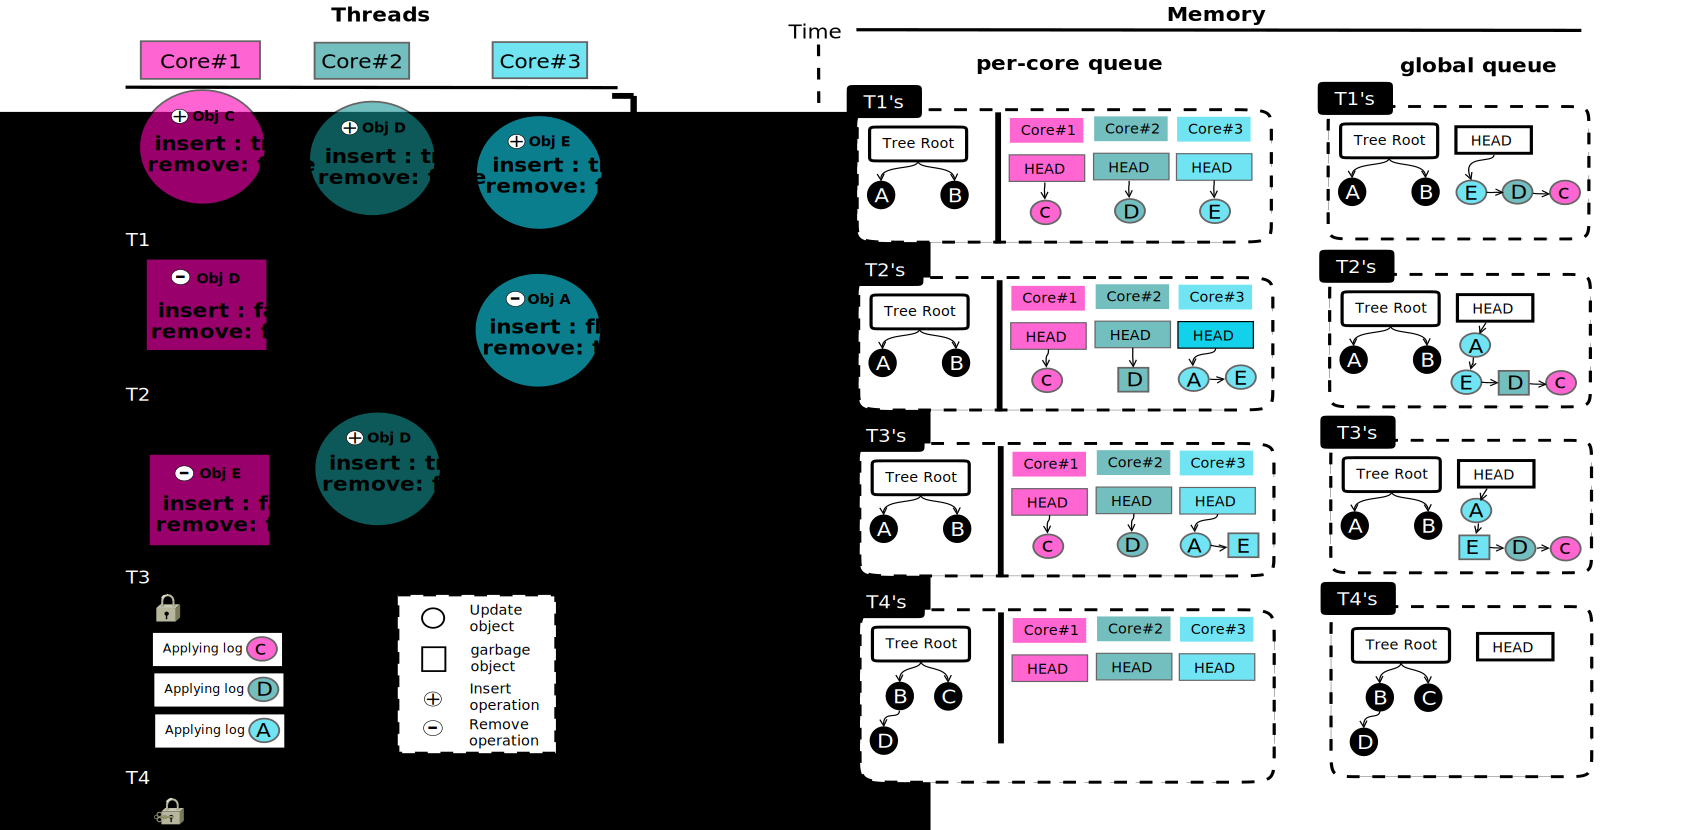
\includegraphics[width=1.0\textwidth,height=0.4\textheight]{fig/basic_gldu}
  \end{center}
  \caption{7개의 업데이트 연산과 1개의 리드 연산에 대한 LDU 예.}
  \label{fig:basic}
\end{figure}

%$$$$$$$$$$$$$$$$$$$$$$$$$$$$$$$$$$$$$$$$$$$$$$$$$$$$$$$$$$$$$$$$$$$$$$$$$$$$$$$$
%Paragraph 1: Flowchart 구조 설명 
%$$$$$$$$$$$$$$$$$$$$$$$$$$$$$$$$$$$$$$$$$$$$$$$$$$$$$$$$$$$$$$$$$$$$$$$$$$$$$$$$

그림 \ref{fig:basic}는 LDU가 퍼코어 큐와 전역 큐를 사용하여 수행되는 예를 보여준다.
높은 업데이트 비율을 가지는 자료구조와 함께, 동시적 지연 업데이트 방법을 설명하고, 
7개의 업데이트 연산들이 읽기 연산 전에 어떻게 동시적으로
수행되는 지를 보여준다.
업데이트 연산의 순서는 다음과 같다. 
\begin{center}
$\oplus$\inv{1}{C}, $\oplus$\inv{2}{D}, $\oplus$\inv{3}{E},$\ominus$\inv{1}{D},
$\ominus$\inv{3}{A}, $\oplus$\inv{2}{D}, $\ominus$\inv{1}{E}. 
\end{center}.
우리는 LDU를 설명하기 위해서 앞 절에서 사용한 심볼에 사각형 모양을 추가하였다. 
즉, 오브젝트 D가 마크필드는 \textit{false}이나 큐에는 여전히 존재하는 오브젝트면 \res{1}{D}로 표시한다.

이 그림에서 실행 순서는 위에서 부터 아래로 이루어진다.
그림 왼쪽에 있는 것은 CPU의 연산들을 보여주고 오른쪽에 있는 것은 특정한 시간에 메모리에 존재하는 
자료구조의 내용에 대해서 보여준다. 
초기 트리 자료구조에는 오브젝트 \inv{0}{A}와 \inv{0}{B}가 들어 있고 큐는 비어 있게 된다.
%$$$$$$$$$$$$$$$$$$$$$$$$$$$$$$$$$$$$$$$$$$$$$$$$$$$$$$$$$$$$$$$$$$$$$$$$$$$$$$$$
%Paragraph 2: Flowchart 그림 설명 
%$$$$$$$$$$$$$$$$$$$$$$$$$$$$$$$$$$$$$$$$$$$$$$$$$$$$$$$$$$$$$$$$$$$$$$$$$$$$$$$$
그림에서 \code{Core\#1}, \code{Core\#2} 그리고 \code{Core\#3}은 
퍼코어 또는 전역 큐에 동시적 업데이트 연산을 수행될 수 있다.
따라서 $\oplus$\inv{1}{C}, $\oplus$\inv{2}{D} 그리고 $\oplus$\inv{3}{E}는 락이 없이 수행된다.

LDU는 연산에 대한 로그를 저장하기 위해 논블락킹 큐를 사용하기 때문에, 
이 작업에는 업데이트 락이 필요 없다. 
따라서 모든 스레드는 락에 대한 경쟁 없이 동시적으로 수행된다. 
\code{T1} 시점이 되면, 트리는 여전히 오브젝트 \inv{0}{A}과 \inv{0}{B}이 존재한다.
그리고 퍼코어 큐와 전역 큐는 오브젝트 $\oplus$\inv{1}{C}, $\oplus$\inv{2}{D} 그리고
$\oplus$\inv{3}{E}가 보관되고, 퍼코어 큐는 퍼코어 메모리에 각각 구별되어 로그가 저장된다.

다음 연산들은 $\ominus$\inv{1}{D}과 $\ominus$\inv{3}{A}이며,
먼저 $\ominus$\inv{1}{D} 연산이 실행이 되면, LDU는 새롭게 로그를 생성하여 큐에 로그를 넣지 않고, 
원자적으로 오브젝트에 있는 마크 필드를 수정한다. 
그리고 $\ominus$\inv{3}{A}은 새로운 연산이기 때문에 큐에 바로 저장한다. 
\code{T2} 시점이 되면, 퍼코어 큐와 전역 큐에는 $\oplus$\inv{1}{C}, $\oplus$\res{2}{D},
$\oplus$\inv{3}{E} 그리고 $\ominus$\inv{3}{A} 로그들이 저장된다. 
이 시점에서는 오브젝트 \res{2}{D}의 삽입에 대한 상태 변수인 마크 필드는 \textit{false}이다. 
이 로그는 업데이트 시점에 삭제된 로그를 의미한다.

마지막 연산들은 $\oplus$\inv{2}{D}, $\ominus$\inv{1}{E} 이다. 
LDU는 원자적 스왑을 사용하여 큐에 있는 로그를 새롭게 생성하지 않고 기존 로그를 다시 재활용한다. 
그러므로, 업데이트 순간 로그 \res{2}{D}는 \inv{2}{D}로 바뀌고, 그리고 로그 \inv{3}{E}는 \res{3}{E}로
수정된다.
\code{T3} 시점이 되면, 퍼코어 큐에는 $\oplus$\inv{1}{C}, $\oplus$\inv{2}{D},
$\ominus$\inv{3}{A} 그리고 $\oplus$\res{3}{E}가 저장된다. 
다음으로, 읽기 함수가 수행되기 전에 트리의 연산들을 보호하기 위해서, 상호배재 기반의 트리 락이 필요하다. 
따라서 LDU는 락을 수행하고, 큐에 저장되어 있는 업데이트 연산들을 단일 스레드에서 모두 수행한다. 
이 때 수행될 연산들은 마크 필드가 \textit{true}로 표시된 로그들이다.
그러므로, 연산 $\oplus$\inv{1}{C}, $\oplus$\inv{2}{D} 그리고 $\ominus$\inv{3}{A}
들이 수행되며 마크 필드가 \textit{false}인 로그인 $\oplus$\res{3}{E}는 수행되지 않는다. 
T5시점이 되면, 트리는 \inv{0}{B}, \inv{0}{C} 그리고 \inv{0}{D}가 존재하게되며, 
최종적으로 리더는 결국 일관성 있는 데이터를 읽게 된다.

\begin{figure}[h!]
\begin{center}
\inputminted[linenos,fontsize=\footnotesize, tabsize=4]{c}{src/ldu_logical_a.c}
\end{center}
\caption{LDU의 동시적 삽입에 대한 알고리즘.}
\label{fig:gldulogicalupdatei}
\end{figure}


\begin{figure}[h!]
\begin{center}
\inputminted[linenos,fontsize=\footnotesize, tabsize=4]{c}{src/ldu_logical_b.c}
\end{center}
\caption{LDU의 동시적 삽제에 대한 알고리즘.}
\label{fig:gldulogicalupdater}
\end{figure}


\subsection{알고리즘}

\subsubsection{로그 삽입}
%$$$$$$$$$$$$$$$$$$$$$$$$$$$$$$$$$$$$$$$$$$$$$$$$$$$$$$$$$$$$$$$$$$$$$$$$$$$$$$$$
%Paragraph 1:LDU Concurrent Updates 알고리즘 코드 및 설명 
%$$$$$$$$$$$$$$$$$$$$$$$$$$$$$$$$$$$$$$$$$$$$$$$$$$$$$$$$$$$$$$$$$$$$$$$$$$$$$$$$
그림 \ref{fig:gldulogicalupdatei}과 \ref{fig:gldulogicalupdater}는 동시적 업데이트를 수행하는
함수에 대해서 보여준다.
동시적 업데이트 함수는 3가지 단계로 구분된다.
첫 번째 단계는 체크 단계이며, 입력으로 받은 오브젝트가 취소 가능한 오브젝트인지 아닌지 확인을 한다(Line 3). 
또한 이 코드는 리더에 의해 아니면 주기적인 함수에 의해 언제든지 \code{synchronize} 함수가 동시에 호출될 수 있다. 

따라서 이 단계에서는 반드시 원자적 명령어인 스왑을 사용한다.
그리고 만약 그에 상응하는 마크 필드가 \textit{true}라면 그것에 대한 마크 필드는 스왑 명령어로 \textit{false}로
수정한다.
두 번째 단계에서는 로그가 이미 큐에 들어가 있는 로그인지 아닌지 체크를 한다(Line 6).
만약 그렇다면, 마크 필드는 이미 \textit{true}로 마크가 되었기 때문에(Line 4), 이 함수는 바로 종료한다.
마지막 단계에서는, 만약 해당연산의 로그가 처음 사용된 로그(Line 9)이면 로그는 논블락킹 큐에 저장한다.

\subsubsection{로그 적용}

\begin{figure*}[h]
\begin{center}
\inputminted[linenos,fontsize=\footnotesize, tabsize=4]{c}{src/ldu_physical.c}
\end{center}
\caption{로그를 적용하는 알고리즘.}
\label{fig:glduphysicalupdate}
\end{figure*}


%$$$$$$$$$$$$$$$$$$$$$$$$$$$$$$$$$$$$$$$$$$$$$$$$$$$$$$$$$$$$$$$$$$$$$$$$$$$$$$$$
%Paragraph 2:LDU Deferred Updates 알고리즘 코드 및 설명 
%$$$$$$$$$$$$$$$$$$$$$$$$$$$$$$$$$$$$$$$$$$$$$$$$$$$$$$$$$$$$$$$$$$$$$$$$$$$$$$$$
그림 \ref{fig:glduphysicalupdate}는 연산에 대한 로그 들을 원본 자료구조에 적용하는 지연 업데이트 함수를 보여준다. 
\code{synchronize} 함수는 읽기 전에 호출되거나 주기적으로 호출되는 타이머 핸들러(timer handler)에 의해
호출된다. 
그 이유는 무한정 로그의 사이즈가 커지는 문제를 방지하기 위해서 이다.
\code{synchronize} 함수는 반드시 오브젝트의 락을 사용하여 반드시 잠금 상태로 되어 있어야 한다.
즉 \code{synchronize} 함수가 수행하기 전에 반드시 락을 잠그는 함수가 호출되어야 한다.
따라서 이 함수는 락에 의해 단일 소비자로 수행된다. 
이 방법은 OpLog의 배치 업데이트(\textit{batching updates})와 FC의 컴바이너 
스레드(\textit{combiner thread})와 유사한 일을 수행한다. 
\code{synchronize} 함수는 제일 먼저 큐의 헤드 포인터를 원자 적인 스왑 명령(Line 3)을 이용하여 
얻는다.
LDU는 주기적으로 로그의 큐의 로그들을 적용하기 때문에, LDU의 업데이트 연산들은 \code{synchronize} 함수와 
동시에 수행될 수 있다. 
그러므로 원본 자료구조에 적용하기 전에 마크필드는 \textit{false}로 수정된다(Line 8,9).
또한 사용이 끝나면 해당 로그를 삭제하기 위한 사용 플래그는 \textit{false}로 수정된다. 
이것은 이 오브젝트가 큐에 포함되어 있지 않는다는 것을 의미한다(Line 10).
\code{synchronize} 함수는 한 번 더 마크 필드가 적용하는 과정(Line 8)과 로그를 재활용하는 과정(Line
10)에서 누군가 로그를 수정하였는지 다시 한번 더 체크를 한다(Line 12,13).

